% ============================================================
%  深圳大学实验报告模板(SZU Experiment Report Template)
% This template can be modified according to the specific requirements of your experiment or project.
% Produced by: Chao Fan and Kewei Ou, AI School of SZU
% ============================================================

\documentclass[a4paper,12pt]{article}

% ----------------------------
% 中文与字体支持
% ----------------------------
\usepackage{fontspec}    % 字体支持
\usepackage{xeCJK}       % 中文字体支持
\setCJKmainfont{Noto Serif CJK SC} % 设置中文字体(Overleaf自带Noto字体)
\usepackage{graphicx}
\usepackage{subcaption}

% ----------------------------
% 页面设置与常用宏包
% ----------------------------
\usepackage{geometry}    % 页面边距控制
\geometry{left=1in, right=1in, top=1in, bottom=1in}

\usepackage{longtable}   % 支持长表格
\usepackage{graphicx}    % 插入图片
\usepackage{fancyhdr}    % 页眉页脚控制
\usepackage{tikz}        % 绘制框线等图形
\usetikzlibrary{calc}    % 坐标计算
\usepackage{verbatim}    % 显示代码块
\usepackage{float}       % 控制图片浮动位置([H]参数)

% ----------------------------
% 页眉页脚设置
% ----------------------------
\pagestyle{fancy}
\fancyhf{} % 清空默认页眉页脚
\fancyhead[L]{深圳大学实验报告} % 左侧页眉文字
\fancyhead[C]{} % 中间空
\fancyhead[R]{} % 右侧空

% ============================================================
%                      文档开始
% ============================================================

\begin{document}

% ============================================================
% 封面页
% ============================================================
\begin{titlepage}
    \centering
    \vspace*{2cm}
    \Huge{\textbf{深 \ 圳 \ 大 \ 学 \ 实 \ 验  \ 报 \ 告}}\\[1.5cm]
    
    \Large{课程名称:\underline{\hspace{2cm}Python程序设计基础\hspace{1.5cm}}}\\[0.5cm]
    \Large{项目名称:\underline{\hspace{1cm}鸢尾花数据分类与可视化\hspace{1.5cm}}}\\[0.5cm]
    \Large{学 \quad \quad 院:\underline{\hspace{2.75cm}人工智能学院\hspace{2.75cm}}}\\[0.5cm]
    \Large{专 \quad \quad 业:\underline{计算机科学与技术(IEEE荣誉班)}}\\[0.5cm]
    \Large{指导教师:\underline{\hspace{4cm}樊超\hspace{4cm}}}\\[0.5cm]
    \Large{报告人:\underline{\hspace{0.5cm}陈泓佳\hspace{0.5cm}} \hspace{0.5cm} 学号:\underline{\hspace{0.5cm}2024104023\hspace{1cm}}}\\[0.5cm]
    \Large{实验时间:\underline{\hspace{2.25cm}2025年11月26日\hspace{2cm}}}\\[0.5cm]
    \Large{提交时间:\underline{\hspace{2.25cm}2025年12月6日\hspace{2cm}}}\\[1.5cm]

    \vfill
    \Large{教务处制}
\end{titlepage}

\newpage

% ============================================================
% 正文部分
% ============================================================
% Experiment Objectives
% Figure
\begin{figure}[t]
    \centering
    \includegraphics[width=0.92\linewidth]{figs/flowchart.png}
    \caption{所有任务的具体步骤(4-2与4-1雷同 不展示)}
    \label{fig:vit-arch}
\end{figure}

\section{实验目的}
本实验旨在解决数据分类与可视化问题,使用sklearn.dataset中自带的鸢尾花数据集作为示例。本实验一共包含四个任务:
\begin{enumerate}
    \item [任务1]:使用不同的分类器,进行两特征三分类,并绘制出相对应的概率密度图。
    \item [任务2]:选择分类器进行三特征两分类,并绘制出决策平面图。
    \item [任务3]:选择分类器进行三特征两分类,并绘制出概率密度图。
    \item [任务4]:选择分类器进行三特征三分类,并绘制出决策曲面图和概率密度图。
\end{enumerate}

% Experiment Process
\section{总体概览}
该实验的整体风格如preview\_of\_data.py所示
\begin{enumerate}
    \item[任务1]:对每个分类器都作一次回归分类,画四个图,前三个图为每类对应的概率密度图,第四个图为总体分类概率密度图。
    \item[任务2]:对3D图像上的网格点进行回归分类,获取分类系数从而得到平面方程作图。
    \item[任务3]:绘制3D图像,x、y轴分别是两个特征,z轴是每个(x,y)对应的概率的Logit表示。绘制出曲面图后,绘制其投影。
    \item[任务4]:对于每个类别都绘制出一个决策曲面从而对整体进行分类。4-1和4-2是同一个子任务的不同表现形式。4-3是第二个子任务,每次固定一个特征作为切片,每次取切片特征的低中高值绘制三个3D图,对于每个切片特征,都有三个类的概率密度图,也即每次都会绘制出9个图,一共绘制3次。
    
\end{enumerate}

% Implementation Details
\section{实验步骤}
本处具体的步骤都展示于图片~\ref{fig:vit-arch}中。由于4-2只是4-1换了个表达方式,不再赘述。接下来讲一些实验亮点: 
\begin{enumerate}
    \item[Part 1]:如图片所示,除了任务1以外,其余任务均无要求要选择哪个分类器,鉴于严谨角度考虑,每次使用模型前我都会验证其正确性(4-3无验证是因为其与4-1使用同种分类器进行同样的分类)。
    \item[Part 2]:4-1中由于渲染了3个曲面导致图像变得非常非常卡,我做了如下措施进行补救:1. 在绘制完曲面后任意取其一个切片查看分类情况,并打印混淆矩阵,经检验,分类结果无大问题。2. 创造了4-2,4-2采用了点云的方式进行绘制,虽然部分牺牲了视觉上的效果,但提高了分类结果的可视性。
    \item[Part 3]:4-3拓展了任务3的思路。任务3也是分别取每一个特征作为切片,每一个切片分成低中高值来绘制。与任务3不同的是,任务3的Logit的正负值就能表示结果(二分类)。但是4-3是三分类,所以4-3的Logit含义与任务3有所不同,4-3对于每一个类都有一个logit,正值则表示属于这个类的概率超过50\%,反之亦然。所以4-3比任务3又多出了3倍数量的图像,我用了分画布展示的方式,使得其视觉上令人感觉比较舒服。
\end{enumerate}

\section{实验结果}
部分实验结果如图所示,注意:并非全部实验结果。
\begin{figure}[htbp]
\centering

% 第一行 3 张
\begin{subfigure}{0.3\textwidth}
\centering
\includegraphics[width=\linewidth]{figs/part1_of_mission4-3.png}
\caption{Part 1 of Mission 4-3}
\end{subfigure}
\begin{subfigure}{0.3\textwidth}
\centering
\includegraphics[width=\linewidth]{figs/part2_of_mission4-3.png}
\caption{Part 2 of Mission 4-3}
\end{subfigure}
\begin{subfigure}{0.3\textwidth}
\centering
\includegraphics[width=\linewidth]{figs/part3_of_mission4-3.png}
\caption{Part 3 of Mission 4-3}
\end{subfigure}

\vspace{0.3em}

% 第二行 2 张
\begin{subfigure}{0.45\textwidth}
\centering
\includegraphics[width=\linewidth]{figs/mission1.png}
\caption{Mission 1}
\end{subfigure}
\begin{subfigure}{0.45\textwidth}
\centering
\includegraphics[width=\linewidth]{figs/mission2.png}
\caption{Mission 2}
\end{subfigure}

\vspace{0.3em}

% 第三行 2 张
\begin{subfigure}{0.45\textwidth}
\centering
\includegraphics[width=\linewidth]{figs/mission3.png}
\caption{Mission 3}
\end{subfigure}
\begin{subfigure}{0.45\textwidth}
\centering
\includegraphics[width=\linewidth]{figs/mission4-1.png}
\caption{Mission 4-1}
\end{subfigure}

\caption{七张图片的整体展示}
\end{figure}


\section{讨论}
本次实验我们学会了如何对一个数据集进行可视化,由上述结果看来我已经基本掌握了可视化的基本步骤。然而本次实验确实仍有不足之处,比如实验4-3中你会发现,其投影只有xOy面的投影(当然xOy面投影已经展示了基本上所有有用信息),原因是因为不知道为什么,我明明使用了和任务3一样的投影方式,4-3的侧面投影颜色总是出现错误,与AI交互多次也无果。但总体而言,每个可视化图像均可以清晰地展示数据的分类以及决策边界,也算是圆满完成任务。此代码已上传至GitHub,链接为https://github.com/ZSZH12138/Python-homework2。

\newpage

% ============================================================
% 批阅与成绩评定页
% ============================================================

% 绘制正文外框(包含批阅区域)
\begin{tikzpicture}[remember picture, overlay]
  \draw[thick] 
    ($(current page.north west)+(2cm,-3cm)$) 
    rectangle 
    ($(current page.south east)+(-2cm,2.5cm)$);
\end{tikzpicture}

\vspace{1cm}

% 批阅区
\noindent \textbf{指导教师批阅意见:}
\vspace{5cm}
\hfill

\vspace{1cm}

\noindent \textbf{成绩评定:}
\vspace{2cm}
\hfill

\vspace{1cm}

\noindent \textbf{指导教师签字:}
\vspace{2cm}
\hfill

\vspace{1cm}

% 备注部分
\noindent \textbf{备注:}
\begin{itemize}
    \item 报告内的项目或内容设置,可根据实际情况加以调整和补充。
    \item 教师批改学生实验报告时间应在学生提交实验报告时间后 10 日内。
\end{itemize}

% ============================================================
%                      文档结束
% ============================================================

\end{document}
